\chapter{Security analysis: case study of D-Link DCS-2130}
\label{chap:cam-dcs}

\section*{Introduction}
\label{sec:dcs-intro}

As part of this thesis, it has been decided to analyse the security aspects of one model of wireless digital camera, the D-Link DCS-2130.
The camera has been selected as being recently released (2011), having good reviews, a large choice of features\footnote{Technical details about the device can be found on D-Link website at \url{http://www.dlink.com/}} and being at reasonable price range (around €100).
No previous security researches were found to be done on this model of camera.
The aim was to select a common camera and take it as a representative example of the personal wireless camera market.\\

\begin{figure}[h]
  \centering
  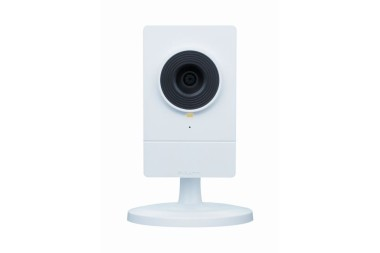
\includegraphics[width=6cm]{images/dcs2130.png}
  \caption{D-Link DCS-2130 camera}
  \label{fig:dcs2130}
\end{figure}

Some of the vulnerabilities and security aspects analysed in this chapter are specific to this model of camera.
However, as weaknesses have been discovered on other models of cameras (as showed the TRENDnet hack), it is believed similar issues can be discovered in other models.\\

\section{DCS-2130 features}
\label{sec:dcs-pres}

The selected camera model is a D-Link DCS-2130 and is represented in Figure \ref{fig:dcs2130}. The camera supports the following protocols:\\

\begin{itemizealt}
\item Wifi: Open, WEP, WPA, WPA2
\item Admin interface: HTTP, HTTPS
\item Access: UPnP, DDNS
\item Transfer: FTP, SMTP, Samba, RTSP
\item Video: H.264, MPEG-4, MJPEG
\item Audio: G.726
\end{itemizealt}

The DCS-2130 has also features such as motion detection allowing to program conditional chains of events (eg: if a motion is detected, upload current pictures to a FTP server).
The camera is provided with an installation utility to configure it from a computer to be able to connect to the wireless network.
% TOCHECK correction "and can be configured blabla
Watching the video stream and configuration of the system can be done using a web interface.
%A software to watch several video streams of different personal cameras without requiring the usage of the admin interface.

\section{Firmware source code}
\label{sec:dcs-gpl}

As many embedded devices, D-Link uses a Linux kernel and open source software such as Busybox which are released under a GPL licence.
A clause in this licence requires to make available the source code of the software using code under GPL if binaries are proposed (which is the case of D-Link).
In 2006, the Court of Frankfurt issued that D-Link was violating the GPL licence on a network-attached storage device~\cite{dlink-gpl-viol}.
Following that ruling, D-Link published the source code of several of their devices on their website\footnote{D-Link GPL Source Code Support \url{http://tsd.dlink.com.tw/GPL.asp}} including the DCS-2130.\\

Even if D-Link technically provides the source code of the software on their website, many difficulties have been faced to obtain the archive file.
The difficulties were:

\begin{itemizealt}
\item No direct link to the file download (impossible to restart an interrupted download)
\item Download speed highly throttle (from 1 to 60Kb/s max.)
\item Regular connection timed out
\item The contact email address provided for this section of the website is invalid
\item No answer while using the general contact form
\end{itemizealt}

Given the nature of the difficulties, one can question if they are intentional to avoid the spreading of the source code too easily.
The source code has finally been retrieved\footnote{The archive downloaded is available on a public FTP server at \url{ftp://ftp.dotzero.me/DLink/}} and the analysis permitted a better understanding of the firmware mechanism as well as the discovery of security issues.

\section{Installation procedure}
\label{sec:dcs-install}

\subsection{Admin account}

The installation and configuration of the software are realised using an ActiveX wizard utility provided with a CD-ROM included with the camera.
This utility is used to configure the connectivity aspect of the camera and to secure the admin account.
The administrator account is used to manage the configuration settings of the camera through the web interface.\\

This last point is positive as the procedure does not permit the configuration of the camera without setting a control access mechanism.
%To access the main web interface, a username and password are required, preventing any unauthorised access to the interface.
However, this control access mechanism is not strong enough to prevent unauthorised visioning as detailed in Section \ref{sec:dcs-guest}.

\subsection{Clear-text authentication}
\label{sec:dcs-clearauth}

At the launch of this wizard, messages broadcasted are exchanged to discover the presence of compatible cameras.
These messages use a proprietary protocol but understandable to anybody listening to the traffic.
The problem of this protocol is the fact that, in the case the camera already is configured for the first time, the authentication of the admin account is required and this communication is also broadcasted, communicating the administrator password in clear text over the network.\\

Below are parts of an exchange between a laptop using the utility and the camera.

{\scriptsize
\begin{verbatim}
   Laptop
0000  ff ff ff ff ff ff 08 00  27 07 34 7d 08 00 45 00   ........ '.4}..E.
0010  00 32 00 33 00 00 80 11  78 d6 c0 a8 01 0a ff ff   .2.3.... x.......
0020  ff ff 04 04 f6 00 00 1e  a2 fc fd fd 01 00 a1 00   ........ ........
0030  ff ff ff ff ff ff 00 00  00 00 00 00 01 00 00 00   ........ ........

   Camera
...
0080  44 4c 69 6e 6b 43 61 6d  00 00 00 00 00 00 00 00   DLinkCam ........
...
00c0  44 43 53 2d 32 31 33 30  00 00 00 00 00 00 00 00   DCS-2130 ........
00d0  00 00 00 00 00 00 00 00  00 00 00 00 00 00 00 00   ........ ........
00e0  31 2e 32 36 00 00 00 00  00 00 00 00 00 00 00 00   1.26.... ........
00f0  00 00 00 00 00 00 00 00  00 00 00 00 00 00 00 00   ........ ........
0100  01 00 27 00 00 00 f0 7d  68 09 52 52 44 4c 69 6e   ..'....} h.RRDLin
0110  6b 43 61 6d 00 00 00 00  00 00 00 00 00 00 00 00   kCam.... ........
...
0140  00 00 00 00 00 00 00 00  00 00 00 00 c0 a8 01 07   ........ ........
0150  50 00 02 00 ff ff ff 00  c0 a8 01 01 c0 a8 01 01   P....... ........
0160  00 00 00 00 01 32 30 31  32 30 36 32 38 30 36 35   .....201 20628065
0170  31 34 34 00 00 42 00 ff                            144..B..         


   Laptop (after giving the credentials to the software)
0000  ff ff ff ff ff ff 08 00  27 07 34 7d 08 00 45 00   ........ '.4}..E.
0010  00 b2 00 34 00 00 80 11  78 55 c0 a8 01 0a ff ff   ...4.... xU......
0020  ff ff 04 05 f6 00 00 9e  82 f7 fd fd 02 00 a3 00   ........ ........
0030  f0 7d 68 09 52 52 c0 a8  01 07 77 77 01 00 80 00   .}h.RR.. ..ww....
0040  59 57 52 74 61 57 34 3d  00 00 00 00 00 00 00 00   YWRtaW4= ........
...
0080  62 58 6c 77 59 58 4e 7a  00 00 00 00 00 00 00 00   bXlwYXNz ........
...
\end{verbatim}
  }


Where \texttt{YWRtaW4=} is \texttt{admin} in base64 encoding and \texttt{bXlwYXNz} is \texttt{mypass}.
These were the username and the password of the camera at the time of the experiment.
While the meaning of each byte would require a larger study, it is however easy to guess the structure of the communication based on the observation:

\begin{enumerate}
\item Laptop: Broadcast detection message
\item Camera: Broadcast presence, model and configuration state
\item The software asks for the administration credentials
\item Laptop: Broadcast the credentials
\end{enumerate}

%Updating the administrator password follows the same 
The fact that all messages are broadcasted implies that, even on encrypted network using session keys such as WPA (which prevents from monitoring the traffic of other users on a wireless network), the credentials are publicly transmitted.
An attacker only needs to monitor the network to be able to retrieve an administrator access to the camera.
However, the use of the utility to reconfigure the network is supposed to be very rare and minimise the risk of such attack.

\section{Security against traffic monitoring}
\label{sec:dcs-proto}

As mentioned in Section \ref{sec:dcs-pres}, the camera supports several protocols.
These protocols are not all as secure and while only monitoring the network an attacker could retrieve sensible information.\\

The monitoring of a network using free tools such as \emph{tcpdump} is possible while an attacker is connected to the same network as the camera and when the wireless network traffic is not encrypted or using WEP\footnote{Unlike WPA/WPA2, WEP does not use unique session keys for each user.}.
On encrypted traffic, an attacker could apply an ARP spoofing attack to force the traffic to transit by its computer and read the content of packages.

\subsection{HTTP authentication}

The access to the web interface allows to watch the video stream but also configure the camera.
This page is protected with a basic authentication mechanism over HTTP.
This authentication is not secured as the credentials are sent in clear text in the headers of the request.
The code below is extracted from the headers of a request to the web interface which contain \texttt{admin:mypass} in base64 encoding.

{\scriptsize
\begin{verbatim}
GET / HTTP/1.1
Authorization: Basic YWRtaW46bXlwYXNz
\end{verbatim}
}

\subsection{URL parameters}

To configure the access to external services (email, FTP, DDNS, etc.) the administrator uses the web interface.
This interface is accessed by default using HTTP which means that the URL of the requested pages is in clear text on the network.\\

For each configuration request, the URL in the headers contains the information for the selected service.
For example, a request to update the password of the wireless access point credential would look like:
{\scriptsize
\begin{verbatim}
GET /cgi-bin/wifi_config.cgi?enable=1&ssid=MyWifiNetwork&Mode=0&\
   auth=3&encrypt=2&wpa_key=MyWifiPassword HTTP/1.1
\end{verbatim}
}

This means that, even if other protocols are secured (eg: usage of SSL in SMTP), the configuration may be the source of information leakages.\\

\subsection{Export configuration}
\label{sec:dcs-config}

The camera features a capability to backup the configuration of the camera, by exporting current settings and information stored in the camera.
In the administration panel on the web interface, the functionality \emph{Save configuration} generates a text file containing all the specified information.
This file contains, in clear text, all the passwords and login information specified during the configuration (user accounts, wireless access, mail credentials, etc.).\\

Apart from the fact that it is worrying that all this information is unnecessarily stored in clear text instead of an encrypted version, this also means that monitoring the traffic while a backup is done may reveal the content of the file.
As for the URL parameters, using secured transmission protocols can be useless if the credentials can be retrieved while monitoring the network.

\subsection{SSL certificate as a solution}

\begin{figure}[h]
  \centering
  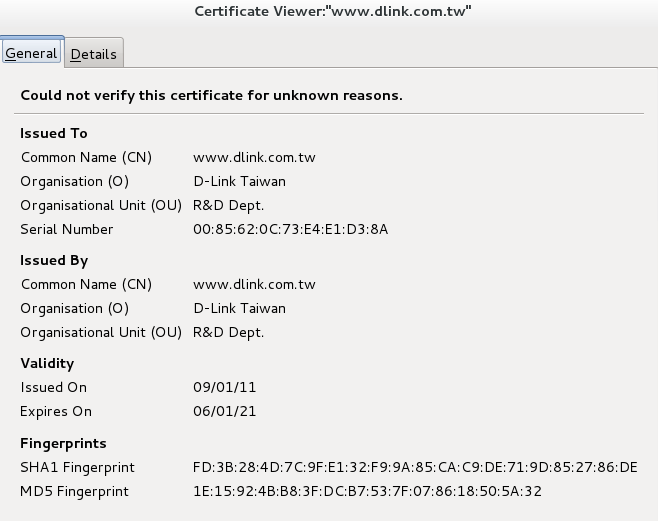
\includegraphics[width=10cm]{images/dcs-ssl.png}
  \caption{Generated self-signed SSL certificate}
  \label{fig:dcs-ssl}
\end{figure}

To prevent the monitoring issues while using the web interface, it is possible to use a SSL certificate to establish a secured HTTPS connection to access the web interface.
However, the certificate used is either self-signed and generated by the camera or uploaded by the user.
Few people will configure an SSL access to the camera but even fewer will have a valid SSL certificate to upload.
It is then very likely that most of the concerned users will use a generated self-signed certificate.\\

In Figure \ref{fig:dcs-ssl}, the imported self-signed generated certificate for the case study camera is displayed in Firefox with a security warning.
This means that an attacker could issue a forged certificate pretending to be the D-Link authority without the possibility for the end user to verify the validity.

\section{Guest account}
\label{sec:dcs-guest}

During the analysis of the camera, it was revealed that the exported configuration file mentioned in Section \ref{sec:dcs-config} contains also the information about the different users allowed to access the camera with their access right level as shown below.

{\scriptsize
\begin{verbatim}
acounts0_name=admin
acounts0_passwd=mypass
acounts0_authority=0
acounts1_name=guest
acounts1_passwd=guest
acounts1_authority=2
\end{verbatim}
}

In this part, an account \emph{guest} using the password \emph{guest} appears with an access level of 2.
This account is automatically created at the installation of the camera.\\

It is important to notice that neither during the installation process nor in the user manual, the existence of a guest account is mentioned.
The only way to detect its presence is to analyse the exported configuration file or see it in the list of removable accounts in the configuration interface (but without knowing the password).
While the obligation to set up a password for the administrator account is positive in terms of security, the hidden creation of the guest account pushes the end user in an incorrect sense of security.

\subsection{Guest account access}
\label{sec:dcs-guest-rights}

The guest account is configured with an access level of two, this level prevents the guest user to modify the configuration of the system but is enough to both watching the video stream and retrieving snapshots of the video using a specific URL.\\

In the firmware source code, the web interface is powered by the open source web server Boa\footnote{Boa Webserver \url{http://www.boa.org/}}.
To resolve the different URLs, this webserver lists all the possible URI with the associated function to execute and the access rights required to access the URI\footnote{In the firmware source code, see \texttt{/apps/public/boa-0.94.13/src/request.c} line 6700}.
Using this list, it is possible to identify what the guest account is capable of.
Fortunately, the guest account appears to be able only to access the stream of the camera and some moderately important information such as the firmware version.

\subsection{Account suppression}
\label{sec:dcs-guest-suppression}

The presence of the guest account is very problematic if a user wants to configure the camera as visible from outside (see Section \ref{sec:dcs-web-access}).
In the administration web interface, it is possible to create and delete users.
However, the removal of the guest account has been specifically prevented.
In the webserver source code, the case of removing the guest user is refused as shown in the code below present in the function responsible for removing an account\footnote{In the firmware source code, see \texttt{/apps/public/boa-0.94.13/src/request.c} line 3280}

{\scriptsize
\begin{verbatim}
...
#ifdef CONFIG_BRAND_DLINK
    else if(i == 1){
       DBG("You can not delete the guest accunt!\n");
       break;
    }
#endif
...
\end{verbatim}
}

This piece of code (typographical error in the original code) is highly surprising as a clear addition from D-Link as an effort to prevent the removal of the guest account (identified by the variable \texttt{i == 1} here).
The reason of this effort is unknown and left to the reader interpretation but it leads to an important security breach as it facilitates the unauthorised viewing of the video stream.\\

As the modification or removal of the guest user is not possible using the web interface, another procedure as been discovered:

\begin{enumerate}
\item Export the configuration file
\item Using a text editor, empty or modify the lines related to the guest account
\item Import the modified file as the new configuration
\end{enumerate}

Emptying the lines will delete the guest account while modifying can keep a guest account present but with a different password.
This procedure is the only known solution to prevent unauthorised access to the web interface using this account.

\section{RTSP protocol}
\label{sec:dcs-rtsp}

The RTSP protocol (for \emph{Real Time Streaming Protocol}) is enabled by default.
As mentioned earlier, this protocol is used to stream the video into another software.
The video stream can be accessed using any compatible third party software using an URL in the form rtsp://\emph{\textless camera-address\textgreater}/\emph{\textless rtsp-path\textgreater}.
Through the admin interface, it is possible to disable, change the port number or rename the access path.\\

Even if technically possible\footnote{The RTSP protocol can implement a basic access control such as it is done on HTTP to access the web interface. However it is not possible to enable this feature on this model of camera.}, the system does not implement any access control mechanism.
If an attacker has access to the associated port (554 by default), it is possible to stream the video, even without necessity to use to the guest account.\\

If not used, it is recommended to disable this protocol.

\section{Log file}
\label{sec:dcs-log}

As mentioned in Section \ref{sec:dcs-guest-rights}, the allowed queries are hard-coded in a list in the file \texttt{request.c} of the webserver.
For some of the requests, there is no execution function associated, only access rights.
This is often the case with requests to the folder \texttt{/cgi-bin/} which contains binary files to execute instead of applying a defined function.\\

During the analysis of the source code firmware, it was noticed that the binary file \texttt{/cgi-bin/exportlog.cgi} was present in the folder of the server but not in the URI list.
This lack of definition in the request file implies that it will be executed according to the file execution rights and not the permissions that could have been defined in the server code.
This means that, even for an anonymous visitor (not guest or admin), it is possible to execute this file.\\

As its name implies, the file exports the log of the camera in a text file.
This log file does not reveal highly sensitive information (no password) but gives the state of camera through time.

{\scriptsize
\begin{verbatim}
2012-05-24 21:01:29 NETWORK LOST
2012-05-24 21:01:29 SD CARD SIZE 7620040 KB
2012-05-24 21:01:34 NETWORK RECONNECT
2012-05-24 21:03:15 admin LOGIN OK FROM 193.44.55.11
2012-05-25 15:40:38 IP CAMERA Received MOTION Trigger
2012-05-25 15:40:41 MOTION STOPPED
\end{verbatim}
}

A more sensitive information displayed in the log file is the login account name, the IP addresses and events such as motion detection activation.
Analysing this information could allow an attacker to retrieve information such as the user habits and presence time.\\

Like the TRENDnet vulnerability showed in Section \ref{sec:trendnet-hack}, the possibility to access the log file is due to a bug and it is not possible for the end user to prevent this security leak.
The only possible mitigation is a regular cleanup of the log file in the administration interface (which few users would normally do).

\section{Web camera discovery}
\label{sec:dcs-web-access}

As mentioned in Section \ref{sec:cam-connect}, it is possible to configure a network to access a camera from outside of the network.
However, this access may create the possibility for attacker to access the camera.
Using the previously mentioned vulnerabilities, intrusions are possible to login as guest account or to access the log file.\\

As mentioned in Section \ref{sec:cam-detection-hidden}, it is possible to scan a network in order to discover hidden IP cameras.
While making a request to an IP address, the headers of the reply are specific to the IP device and make it possible to easily identify the presence of cameras.
The reply headers of a request shown below contains the identifier \texttt{Basic realm="DCS-2130"} which can be used.

{\scriptsize
\begin{verbatim}
HTTP/1.0 401 Unauthorized
Date: Sat, 12 Feb 2011 17:59:32 GMT
Server: Boa/0.94.13
Connection: close
WWW-Authenticate: Basic realm="DCS-2130"
Content-Type: text/html; charset=ISO-8859-1
\end{verbatim}
}

As a proof of contest, the program \texttt{dcs\_detection.py} was developed.
This script scans a given range of IP addresses until it detects a basic realm containing \texttt{DCS-2130}.
In a few minutes, this script can discover the presence of a camera on a home network or on a public IP range.
The example below shows the execution of the script detected two cameras in about 4 minutes on a /24 range of IPs.\\

{\scriptsize
\begin{verbatim}
$ time python dcs-detection.py 78.37.191.x
Iterating on 256 urls

78.37.191.73    --> DCS-2130 camera!
78.37.191.117   --> DCS-2130 camera!

real    3m57.994s
user    0m2.007s
sys     0m0.127s
\end{verbatim}
}

Using Shodan search engine (discussed in Section \ref{sec:shodanhq}) with the keyword \texttt{DCS-2130} is another efficient way to retrieve quickly a list of IPs connected to this model of camera.
Using the developer API, the script \texttt{shodan-dcs.py} has been developed to list the indexed DCS-2130 cameras.\\

Using the list of discovered IPs can be exploited to access video streams as shown in Figure \ref{fig:cam-snapshot}.
Through personal experience, only one camera accessible from the web had the guest account not available but had the RTSP port open.
Bottom line, no DCS-2130 camera found on the web was effectively able to prevent access to the video stream.
This is the consequence of combination of the unknown presence of the guest account and the ease to detect such devices.

\begin{figure}[h]
  \centering
  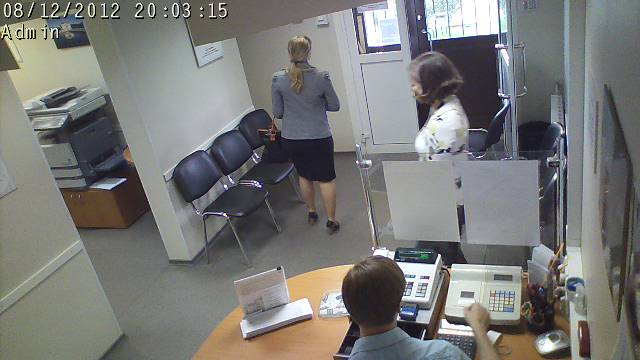
\includegraphics[width=10cm]{images/dms2.jpg}
  \caption{Snapshot from a DCS-2130 discovered while scanning an IP range}
  \label{fig:cam-snapshot}
\end{figure}

\section{PRNG testing}
\label{sec:dcs-random}

Random numbers are used in many security protocols.
The unpredictability of these random numbers are essential to ensure the secrecy while generating keys or initialisation vectors.
The generation of true random numbers is a common challenge in computer sciences as a computer is deterministic.
Instead, devices use arbitrary inputs such as disk moves or network noise to generate pseudo-random numbers.
However, on small embedded devices such as wireless cameras, there is not as many possible inputs as on a personal computer (no hard drive for instance).
A weak random generation procedure may lead to a weak usage of theoretically secured protocols.\\

As a way to evaluate the security of the camera, the quality of the PRNG (Pseudo-Random Number Generator) used by the camera has been verified.
To evaluate the randomness quality of generated numbers, the tests from the NIST were used\footnote{The NIST, \emph{National Institute of Standards and Technology}, provides open source software available at \url{http://csrc.nist.gov/groups/ST/toolkit/rng/index.html}.}.
These tests are a recognised standard and allow to give a neutral evaluation of the security of the PRNG in the camera.\\

To retrieve as many bits of entropy as possible, the program \texttt{gen\_https.py} has been developed.% and is available in the appendix.
This script generates a specified number of SSL connections to the web interface of the camera.
While this script was running, the network was monitored using the tool \emph{tcpdump} recording the communication in the PCAP format.
In each HTTPS connection, each participant of the connection uses a 28 bytes payload of random bytes.
These bytes were extracted from the trace file using another developed script \texttt{pcap\_to\_random.py}.
For each set of requests, the random bytes from the camera and from the laptop used in the experience were separated and evaluated using the NIST tests set.\\

The following methodology was used through the experiment

\begin{enumerate}
\item Start the \emph{tcpdump} utility
\item Run the \texttt{gen\_https.py} with 5000 connections
\item Stop \emph{tcpdump}
\item Extract the bytes of entropy from the camera and the laptop using \texttt{pcap\_to\_random.py}
\item Run the NIST tests on both extracted random sequences and compare the results
\end{enumerate}

The experiment was repeated several times in a row to test the evolution as the pool of entropy of both devices was emptied.
As a set of 5000 connections uses 140Kb of entropy, experiment showed that one run is enough to empty the main pool of randomness on the test laptop.\\

The conclusion of these tests was that, in every tested run, the entropy of both the laptop and the camera were sufficient to pass the NIST tests.
If the tests carried out on the laptop showed better results than the ones using the camera, both were still enough to be considered as random.
The difference between the two devices can be explained by the fact that the camera has no hard drive and more external sources of entropy, allowing it to refill the pool of entropy faster than the camera.

\section{Burglar scenario}
\label{sec:dcs-burglar}

As an example of issues related to lack of security from a wireless camera, the scenario of a burglar (with some computer knowledge) planning to visit a building equipped with a DCS-2130 camera is detailed.
This is one possible abuse showing concretely the danger of forgetting the privacy aspect while using this device.
Another possible abuse for professionals would be industrial espionage.
Two scenarios are discussed in detail below depending of the situation of the burglar.
Not every case may lead to an abuse of the camera.

\subsection{Physically close to the camera}

\begin{figure}[h]
  \centering
  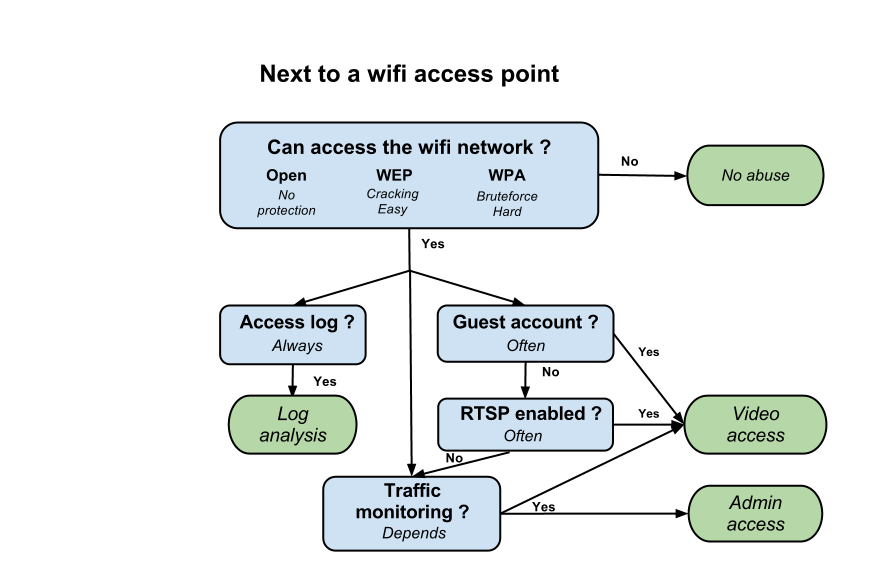
\includegraphics[width=13cm]{images/burglar-inside.png}
  \caption{Case where the burglar is next to the access point}
  \label{fig:burglar-inside}
\end{figure}

This first scenario represented in Figure \ref{fig:burglar-inside} is the case where the burglar is in the range of the wireless camera while planning the visit.
To be able to abuse the camera, it first requires to penetrate the wireless network.
To achieve this goal, the protection of the network is directly related to the feasibility of this step.
In the case of open network or WEP network this is possible easily but if WPA or WPA2 is used, this may be more difficult\footnote{The wifi penetration techniques are not detailed in this section and left to the reader researches.}\\

Once an access to the network is realised, the burglar has three main sources of information:
\begin{enumerate}
\item Access the log to retrieve information such as presence hour of inhabitants, motion detection system, etc. (always possible)
\item Access the video stream using RTSP or the guest account to spy the inhabitants of the building (often possible)
\item Gain an administrator access by monitoring the network for a longer period and abusing from the clear-text messages to retrieve credentials (depending of the possibility to monitor the traffic for an extended period of time)
\end{enumerate}

Gaining an administrator access could be useful for the burglar to be able to disable camera surveillance mechanisms such as motion detection during the future visit.
The access to the video stream also helps the burglar to detect the precise emplacement of the camera and avoid getting caught on tape during his misdeed.

\subsection{Web access to the camera}

\begin{figure}[h]
  \centering
  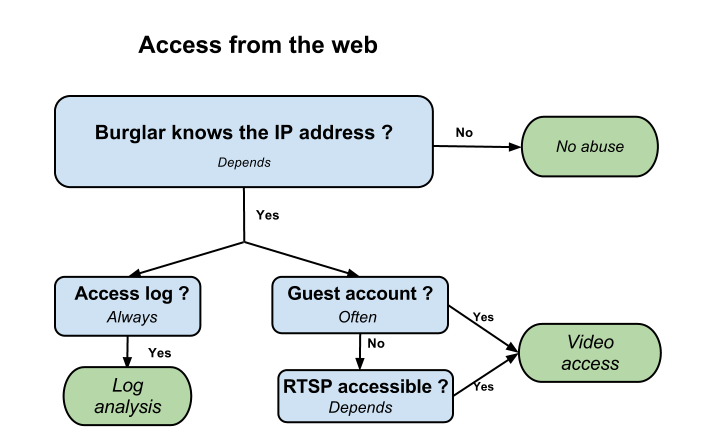
\includegraphics[width=13cm]{images/burglar-outside.png}
  \caption{Case where the burglar access the camera from the web}
  \label{fig:burglar-outside}
\end{figure}

The second abuse case represented in Figure \ref{fig:burglar-outside} is when the camera is accessible from the web using the public IP address.
The requirements are harder to achieve than the previous abuse case as the burglar needs to know the IP address of the targeted house (no other efficient techniques than scanning large IP ranges).
Another possible scenario would be the burglar deciding the visit of a building based on the availability of a camera and obtaining the location based on the observations and IP address.\\

If the requirements are met, two possibilities of abuse are now possible:
\begin{enumerate}
\item Access the log to retrieve information such as presence hour of inhabitants, motion detection system, etc. (always possible)
\item Access the video stream using RTSP or the guest account to spy the inhabitants of the building (often possible)
\end{enumerate}

The RTSP availability is less likely to be possible than in the first case as it requires a full access to the ports of the camera and not a simple port forwarding of the needed port (80 or 443 to access the web interface).
However, during the experiments, some cameras where discovered as fully available from the Internet with the RTSP port open.

\section{Security advises}
\label{sec:dcs-security}
To conclude the camera analysis, the usage of the camera without taking security measures is not considered as safe and is not recommended.
The owners of this model of camera should apply the following steps:

\begin{itemizealt}
\item Disable the guest account.
\item If not used disable the RTSP stream.
\item Secure efficiently the wifi network (WPA or WPA2 with a hard to guess password).
\item Use the web interface in HTTPS after making sure to import the certificate while in a secured environment\footnote{Wired connection, no potential attacker on the network...}.
\item Cleanup regularly the cache file.
\item Avoid configuring the camera when not necessary, especially using the installation utility.
\end{itemizealt}

\section{D-Link reactions}
\label{sec:dcs-dlink}

Before the publication of this thesis, it has been tried to contact D-Link.
Both the contact email address of the Benelux support and the community forum were used to try to establish a discussion with a D-Link member regarding these concerns.
Unfortunately none of the attempted communications have led to an answer.\\

As it is possible the messages did not reach the adequate D-Link members, it is disappointing that it was not possible to contact them before the publication of this thesis.
However, it is hoped that these issues will be noticed by D-Link and be fixed in future version of the firmware.

\section{Future research}
\label{sec:dcs-future}

During the study of the camera, several researches where started but did not reach a conclusion and could be continued in future works.


\subsection{Firmware modification}

As the source code of the firmware was provided, it has been possible to build the source code into an installable image.
Future researches could try to modify the firmware to develop a more hacker-friendly environment and being able to run deeper analysis of the behaviour of the camera while running.

\subsection{Stream interception}

Experiences showed the video traffic is accessible using an ARP spoofing attack.
However, no attack on the traffic has been applied.
A possible attack would be the on-the-fly modification of the video stream while using the RTSP protocol.\\

If technically possible, this attack is difficult to set up due to the complexity and variety of the different video and audio protocols.
A similar attack on Cisco IP surveillance camera has already been demonstrated~\cite{ucsniff}, showing the feasibility of such attack.

\subsection{Port 1010}

While scanning the opened port of the device, every opened port had a clear purpose (HTTP, RTSP, UPnP, etc.) with the exception of the port 1010.
This port is opened but during the tests it was found that this port was never used, nor did it reply to tried queries.\\

A future research could determine what is the usage of this port and his eventual interest in the security analysis of the camera.

\subsection{Other models of cameras}

The discussed issues have been detected for the selected camera.
As the time and resources were limited, only the DCS-2130 model was studied.
However it could be interesting to extend the researches to see if the issues mentioned also apply to other models of camera.
